% ======================================================================================================
% EH627 final project report: The Regional Footprint of AI Data Centres
% Build:  cd report && tectonic -X compile --keep-logs main.tex      (see ../CLAUDE.md for the full loop)
% Figures: report/analysis/*.py -> report/figs/*.pdf     Tables: report/analysis/make_tables.py -> report/tables/
% Text: one file per section in report/sections/. Every number: presentation/data/claims.csv or
%       report/data/claims_report.csv. Status and TODOs per teammate: report/STATUS.md.
% ======================================================================================================
\documentclass[9pt,a4paper]{extarticle}
\usepackage[T1]{fontenc}\usepackage{lmodern}
\usepackage[a4paper,margin=0.70in,headsep=10pt]{geometry}
\usepackage{microtype,amsmath,graphicx,xcolor,booktabs,array,multirow}
\newcolumntype{P}[1]{>{\raggedright\arraybackslash}p{#1}}
\usepackage{caption,fancyhdr,tcolorbox,enumitem,ragged2e,textcomp}
\usepackage[round,authoryear]{natbib}
\usepackage[compact]{titlesec}
\usepackage{stfloats}
\usepackage[hidelinks]{hyperref}
\tcbuselibrary{skins,breakable}

% ---------------------------------------------------------------- draft switch
% \drafttrue shows the red [TODO name: ...] notes for the team. Set \draftfalse for the submitted PDF.
\newif\ifdraft
\draftfalse
\newcommand{\todo}[2]{\ifdraft{\color{red!65!black}\sffamily\scriptsize[TODO #1: #2]}\fi}

% ---------------------------------------------------------------- authors (fill in the placeholders)
\newcommand{\AuthorA}{Aryan Solanki}\newcommand{\RollA}{23110049}
\newcommand{\AuthorB}{Aditya Kumar}\newcommand{\RollB}{22110015}
\newcommand{\AuthorC}{Prerna Sawane}\newcommand{\RollC}{22110235}
\newcommand{\ShortTitle}{The Regional Footprint of AI Data Centres}

% ---------------------------------------------------------------- colours (navy = reference PDF; phases = deck)
\definecolor{navy}{HTML}{12305E}
\definecolor{phaseGA}{HTML}{8C4A2F}\definecolor{phaseCloud}{HTML}{6B7783}\definecolor{phaseAI}{HTML}{2E5EAA}
\newcommand{\phGA}[1]{\textcolor{phaseGA}{\textbf{#1}}}
\newcommand{\phCloud}[1]{\textcolor{phaseCloud}{\textbf{#1}}}
\newcommand{\phAI}[1]{\textcolor{phaseAI}{\textbf{#1}}}

% ---------------------------------------------------------------- layout (playbook section 4b)
\setlength{\columnsep}{0.26in}
\titleformat{\section}{\large\bfseries}{\thesection.}{0.55em}{}
\titleformat{\subsection}{\normalsize\bfseries}{\thesubsection}{0.55em}{}
\titleformat{\paragraph}[runin]{\normalsize\bfseries}{}{0pt}{}[.]
\titlespacing*{\section}{0pt}{7pt}{3pt}
\titlespacing*{\subsection}{0pt}{5pt}{2pt}
\titlespacing*{\paragraph}{0pt}{2pt}{0.5em}
\renewcommand{\topfraction}{0.94}\renewcommand{\bottomfraction}{0.88}
\renewcommand{\textfraction}{0.05}\renewcommand{\floatpagefraction}{0.72}
\renewcommand{\dbltopfraction}{0.94}\renewcommand{\dblfloatpagefraction}{0.72}
\setcounter{topnumber}{3}\setcounter{dbltopnumber}{2}\setcounter{totalnumber}{5}
\setlength{\textfloatsep}{8pt plus 2pt minus 3pt}
\setlength{\intextsep}{7pt plus 2pt minus 3pt}
\setlength{\dbltextfloatsep}{9pt plus 2pt minus 3pt}
\linespread{1.005}
\tolerance=1500\emergencystretch=1.4em\hyphenpenalty=90
\hyphenation{Aque-duct data-centre data-centres Visa-kha-pat-nam Tar-lu-va-da Ada-vi-va-ram Ram-bil-li Ad-ani-Con-neX geo-coded}
\setlist{nosep,leftmargin=1.2em}
\captionsetup{font=small,labelfont=bf,labelsep=colon,justification=justified,singlelinecheck=false}
\captionsetup[table]{position=top,skip=3pt}
\captionsetup[figure]{skip=4pt}

% ---------------------------------------------------------------- header and footer
\pagestyle{fancy}\fancyhf{}
\fancyhead[L]{\footnotesize\color{navy}Final Report \textbar\ EH627}
\fancyhead[R]{\footnotesize\color{navy}\ShortTitle}
\fancyfoot[C]{\footnotesize\thepage}
\renewcommand{\headrulewidth}{0.4pt}
\renewcommand{\headrule}{\hbox to\headwidth{\color{black!30}\leaders\hrule height \headrulewidth\hfill}}

% ---------------------------------------------------------------- call-outs and "our reading" paragraphs
\newtcolorbox{finding}[1]{enhanced,colback=navy!4,colframe=navy,coltitle=white,
  fonttitle=\bfseries\scriptsize,title={#1},boxrule=0.6pt,arc=1.2pt,
  left=4.5pt,right=4.5pt,top=2.5pt,bottom=2.5pt,before skip=5pt,after skip=5pt,fontupper=\small}
\newenvironment{reading}{\par\smallskip\noindent\itshape\small\ignorespaces}{\par\smallskip}

% ---------------------------------------------------------------- bibliography in small type
\setlength{\bibsep}{1.2pt plus 0.3pt}
\renewcommand{\bibfont}{\footnotesize}
\renewcommand{\bibsection}{\section{Bibliography}}

% \tabin{file}: input a generated table body inside a tabular (LaTeX's \input breaks \bottomrule there)
\makeatletter\newcommand{\tabin}[1]{\@@input #1 }\makeatother
\newcommand{\Fig}[1]{Figure~\ref{#1}}
\newcommand{\Tab}[1]{Table~\ref{#1}}
\newcommand{\cotwo}{CO\textsubscript{2}}
\newcommand{\kmc}{km\textsuperscript{3}}

\begin{document}
% ====================================================================================== title page
\pagenumbering{Alph}\thispagestyle{empty}
\begin{center}
\vspace*{1.7cm}
{\large\scshape Final Project Report}\\[2.4cm]
{\LARGE\bfseries The Regional Footprint of\\[3pt] AI Data Centres}\\[12pt]
{\large Energy, Water, Materials and Planetary Boundaries}\\[6pt]
{\normalsize\itshape Three phases since 1950, and why AI growth no longer stays flat}\\[1.6cm]

\includegraphics[width=3.4cm]{iitgn_logo_clean.png}
\vfill
{\renewcommand{\arraystretch}{1.25}
\begin{tabular}{@{}lcl@{}}
\textbf{\AuthorA} & \textbar & \RollA \\
\textbf{\AuthorB} & \textbar & \RollB \\
\textbf{\AuthorC} & \textbar & \RollC \\
\end{tabular}}\\[16pt]
{\normalsize Indian Institute of Technology Gandhinagar}\\[5pt]
{\normalsize Course: EH627 Anthropocene: Human Impact on the Earth}\\[5pt]
{\normalsize Submitted to: Prof.\ S.\ K.\ Tandon and Prof.\ Vikrant Jain}\\[14pt]
{\normalsize November 2026}
\vspace*{1.4cm}
\end{center}
\clearpage
\pagenumbering{arabic}

% ====================================================================================== body page 1
\twocolumn[{%
\begin{center}
{\Large\bfseries The Regional Footprint of AI Data Centres}\\[4pt]
{\small Energy, water, materials and planetary boundaries.
EH627 \emph{Anthropocene: Human Impact on the Earth}, group project, final report}
\end{center}
\vspace{2pt}
\begin{minipage}{\textwidth}\small\noindent% Abstract (all). Full-width paragraph on body page 1. Keep under ~230 words.
\textbf{Abstract.} Every AI model runs in a data centre that draws electricity, evaporates water for cooling and is
built from mined hardware that ends as e-waste. Data centres used about 1.5\% of the world's electricity in 2024, and
the IEA expects that to roughly double by 2030. We place this growth in three phases since 1950 (the Great
Acceleration, the cloud era and the AI era) and ask why cloud growth left data-centre electricity almost flat while AI
growth does not. Combining Epoch AI's 96 AI data centres (15.1\,GW today, 50.3\,GW planned by 2030) with WRI Aqueduct,
the GHSL population grid, Ember, USGS and published energy series, we find that AI training compute broke upward in
2011, but US data-centre electricity only accelerated after 2018 (from about 7\% to 18\% a year), once building
efficiency had stopped improving. Weighted by power, 34\% of tracked AI capacity sits in basins of high or extremely
high water stress today and 39--45\% of the 2030 plan; 21 million people live within 25\,km of those sites. The sites
consume an estimated 143--624 billion litres of water a year, 67--86\% of it at the power plants that supply them.
Against the global freshwater boundary this is under 0.1\%; in Google's Mesa basin, withdrawals already exceed supply in
all twelve months. At the planned Visakhapatnam hub, water risk shaped the cooling design but was not a siting test, and no binding framework required one. Capacity is far more concentrated than people (country-level Gini 0.94), and the minerals come from a
few producing countries. AI's footprint is small globally and concentrated locally, so responses have to be matched to
the local, regional and global scale of each impact.
\end{minipage}
\vspace{9pt}
}]

% 1 Statement of the problem (all; first draft: Aryan). Sources: deck slides 2-6, claims.csv rows S1, S1/O1, S5/O3.
\section{Statement of the problem}\label{sec:problem}

Artificial intelligence is usually discussed as software, but it has a physical body. Every model is trained and run
in a data centre: a building packed with servers whose chips draw electricity, shed heat that has to be removed, often
by evaporating water, and are made of copper, gallium, cobalt and rare earths that are mined in a few places and end up
as electronic waste. In this report ``AI'' means that infrastructure, not the algorithms.

Data centres used about 415\,TWh in 2024, roughly 1.5\% of the world's electricity, and the International Energy
Agency's base case has them reaching about 945\,TWh by 2030 \citep{iea2025}. That growth lands on an Earth system that
is already outside most of its safe operating space. Each assessment of the planetary boundaries has found more of them
crossed: three of seven in 2009 \citep{rockstrom2009}, four in 2015 \citep{steffen2015pb}, six of nine in 2023
\citep{richardson2023} and seven of nine in the latest Planetary Health Check \citep{sakschewski2025,src_pb}. Data
centres press on several of them at once: climate through their electricity, freshwater through cooling and power-plant
water, and novel entities and biosphere integrity through e-waste and mining.

A share of 1.5\% sounds small, and globally it is. But it is not spread evenly. The United States (45\%), China (25\%)
and Europe (15\%) account for 85\% of data-centre electricity \citep{iea2025}, and the large AI sites tracked by Epoch
AI are more concentrated still: 83\% of their 15\,GW is in the United States \citep{epoch2026dc}. The impacts
therefore fall on particular grids, river basins and communities. A recent global study placed one quarter of the
world's data centres in water-stressed areas \citep{rosa2026}, but it counts facilities: a 10\,MW server room and a
2\,GW AI campus count the same, and their water use is not estimated. No assessment we know of weighs data centres by
size and relates them to the water and the people around them. That is the gap this project addresses.

\paragraph{Three phases and one puzzle} We frame the history in three phases since 1950. In the \emph{Great
Acceleration} (1950--2010) energy use, \cotwo\ and material extraction rose together \citep{steffen2015ga}. In the
\emph{cloud era} (2010--2018) computing grew enormously, yet global data-centre electricity barely moved: by one widely
used estimate, compute instances rose by about 550\% while energy use rose by about 6\% \citep{masanet2020}. In the
\emph{AI era} (2019 onward) that decoupling broke: US data-centre electricity rose from 76 to 176\,TWh between 2018
and 2023 \citep{shehabi2024}. Our organising question is therefore: \emph{why did cloud growth leave energy use almost
flat, while AI growth does not?}

\begin{finding}{Terms used in this report}
\textbf{MW and TWh.} Power (MW, GW) is a rate; energy (TWh) is power over time. 1\,GW running all year is about
8.8\,TWh. Epoch AI reports \emph{facility} power, the whole building, not just the computers.
\textbf{PUE} (power usage effectiveness) = facility energy $\div$ IT energy; 1.5 means an extra 50\% goes to cooling
and losses. \textbf{WUE} (water usage effectiveness) = litres of water consumed on site per kWh of IT energy.
\textbf{Grid water intensity} = litres consumed at power plants per kWh generated. \textbf{Withdrawal vs
consumption:} water withdrawn is taken from a river or aquifer, and part is returned; water consumed is evaporated and
lost to the basin. \textbf{Water stress} (WRI Aqueduct) = annual withdrawals as a share of a basin's renewable supply:
above 40\% is \emph{high}, above 80\% \emph{extremely high}.
\end{finding}

% 2 Objectives (all). Source: project plan section 2; deck slides 8-9.
\section{Objectives}\label{sec:objectives}

\paragraph{Broad objective} A diagnosis of \emph{whether}, \emph{where} and \emph{at what scale} AI data centres put
pressure on planetary boundaries, as a basis for responses matched to each scale of impact. The scale matters because
it decides who has to respond: a town council, a grid or river-basin authority, or an international agreement.

\paragraph{Specific objectives} Each objective covers one part of the Earth system and has one owner in the group.
\begin{description}[leftmargin=0pt,labelsep=0.4em,itemsep=1.5pt]
\item[O1 Energy and carbon] (atmosphere; Aditya). Map the regional distribution of data-centre electricity and grid
carbon intensity; compare growth rates across the three phases; explain why the cloud era stayed nearly flat while the
AI era does not.
\item[O2 Materials, water and waste] (hydrosphere and lithosphere; Aryan). Quantify the water-stress exposure of AI
capacity and of the people near it; estimate water use and identify water sources; trace the geography of critical
minerals and e-waste.
\item[O3 Economy, politics and society] (anthroposphere; Prerna). Measure how unevenly capacity is distributed
relative to population; document local opposition and supply-chain concentration.
\item[O4 Synthesis] (all). Place the findings on the planetary boundaries \citep{sakschewski2025} and the
safe-and-just Earth system boundaries \citep{rockstrom2023}, classified by scale of impact: local, regional or
global.
\end{description}

% 3 Data and methods (all; first draft: Aryan). Sources: deck slides 10-14; scripts in presentation/analysis and
% report/analysis. Parameter values: presentation/analysis/water_params.py (claims.csv rows O2c).
\section{Data and methods}\label{sec:methods}

\subsection{Datasets}
\Tab{tab:data} lists the sources actually used. The backbone is Epoch AI's database of AI data centres
\citep{epoch2026dc}: 96 large AI sites with their current facility power and build timelines to the end of 2030. It is
the only open dataset that gives power and timelines site by site. Its coverage is the main limit on what follows
(Section~\ref{sec:limits}): it tracks AI sites only, not all data centres, and most of them are in the United States.

\begin{table}[t]\centering
\caption{Datasets used, by theme. All are public; each number in the report traces to one of them or to our scripts.}
\label{tab:data}
\footnotesize\renewcommand{\arraystretch}{1.08}
\begin{tabular}{@{}P{1.75cm}P{5.85cm}@{}}
\toprule
Theme & Sources \\
\midrule
Sites and capacity & Epoch AI data centres: 96 sites, facility MW today and planned to 2030 \citep{epoch2026dc};
geocoded with OpenStreetMap Nominatim \citep{osm2026} \\
Electricity, efficiency & IEA global and regional, 2024--2030 \citep{iea2025}; LBNL US series 2014--2023
\citep{shehabi2024}; global estimates 2010--2018 \citep{masanet2020}; Uptime PUE survey 2007--2025
\citep{uptime2025} \\
Growth & World primary energy 1950--2019 \citep{owid2026energy}; training compute of 540 notable AI models
\citep{epoch2026models} \\
Carbon & Ember grid carbon intensity by country, 2024 \citep{ember2026} \\
Water & WRI Aqueduct 4.0: baseline annual and monthly stress, 2030 and 2050 projections \citep{kuzma2023}; WUE, PUE
and grid water-intensity ranges \citep{devriesgao2026}; city records and news reports (case studies) \\
Population & GHSL GHS-POP 2025, 30 arc-second grid \citep{schiavina2023} \\
Materials, waste & USGS Mineral Commodity Summaries 2026 \citep{usgs2026}; Global E-waste Monitor 2024
\citep{balde2024} \\
Boundaries & Planetary Health Check 2025 \citep{sakschewski2025}; Earth3 thresholds \citep{collste2018}; Great
Acceleration framing \citep{steffen2015ga} \\
Society & Data Center Watch Q1 and Q2 2026 (US) \citep{dcw2026,dcw2026q2}; EJAtlas grievance categories \citep{temper2015} \\
Siting record & Public statements, official documents and press on the Visakhapatnam hub; Google's 2026 Environmental Report
\citep{google2026env}; NITI Aayog framework \citep{niti2026}; CEEW study \citep{ceew2026} (Section~\ref{sec:siting}) \\
\bottomrule
\end{tabular}
\end{table}

\paragraph{Changes from the plan} The plan proposed a wider net. We used Epoch AI sites only, with no all-data-centre
layer and no footprint-based size model; two case studies instead of three or four clusters, plus a siting audit of the Visakhapatnam hub (Section~\ref{sec:siting}), which was not in the plan; country population from
the GHSL grid rather than UN WPP for the location quotients; no Gini per internet user and no dispute catalogue of our
own; and world primary energy as the only Great Acceleration series.

\subsection{Analytical and statistical methods}

\paragraph{1. Spatial overlay} Each Epoch site was geocoded from its address (all 96 matched, with no country or
state mismatches after restricting queries by country code) and joined to its Aqueduct basin. City-level accuracy is
enough: basins are tens to hundreds of kilometres across. For every site we read the baseline water-stress category,
the 2030 and 2050 projections (business as usual and pessimistic) and the number of months in which withdrawals exceed
supply. The key output is the share of capacity, weighted by MW, in high or extremely high stress, now and for the
planned 2030 capacity. People near the sites were counted from GHSL cells whose centres lie within 25 and 50\,km;
overlapping circles are merged, so nobody is counted twice. The same cells, aggregated by country, are used for the
country table (method 2).

\paragraph{2. Inequality} For each country $i$ with capacity $C_i$ and population $P_i$, the location quotient
\begin{equation}
LQ_i = \frac{C_i / C}{P_i / P}
\end{equation}
is above 1 when a country hosts more than its population share. Countries are then sorted by capacity per person to
draw a Lorenz curve, with cumulative population share $x_k$ and cumulative capacity share $y_k$, and
\begin{equation}
G = 1 - \textstyle\sum_k (x_k - x_{k-1})(y_k + y_{k-1}).
\end{equation}
Countries with no tracked site are pooled into one zero-capacity group. Because they all have exactly zero capacity,
pooling them leaves $G$ unchanged, so this is the exact country-level Gini for the Epoch sample. Country and world
population are sums of GHSL 2025 cells (8.19 billion people), so numerators and denominators come from the same grid.

\paragraph{3. Water-use range} Water is estimated from electricity. With facility power $M$ (MW) and load factor
$L$,
\begin{equation}
E_{\text{fac}} = M L \times 8{,}760\,\text{h},\qquad E_{\text{IT}} = E_{\text{fac}} / \text{PUE},
\end{equation}
\begin{equation}
W_{\text{direct}} = E_{\text{IT}}\times\text{WUE},\qquad W_{\text{indirect}} = E_{\text{fac}}\times WI_{\text{grid}}.
\end{equation}
The low case uses PUE 1.10, WUE 0.56\,L/kWh and $WI_{\text{grid}}$ 1.04\,L/kWh; the high case PUE 1.43, WUE 1.04
and $WI_{\text{grid}}$ 4.52, all from \citet{devriesgao2026}, who compiles IEA, LBNL and company values. The load factor
(70\% low, 90\% high) is \emph{our assumption}: AI clusters run close to continuously, but no site reports its average
draw. Both terms are \emph{consumption}. The low and high cases combine the extremes of each range, so they are bounds,
not a confidence interval.

\paragraph{4. Standardised growth} Each series is fitted as $\ln y_t = a + bt$ by ordinary least squares, giving the
annual growth rate and doubling time
\begin{equation}
r = e^{b} - 1,\qquad T_2 = \ln 2 / b.
\end{equation}
Intervals (95\%) are reported where a yearly series exists; observed and projected years are kept separate. For the
report we added fit diagnostics: $R^2$, the Durbin--Watson statistic for serial correlation in the residuals
\citep{durbin1950}, and a Newey--West standard error for $b$ \citep{newey1987} with
$\lfloor 4(n/100)^{2/9}\rfloor$ lags. Serial correlation leaves the slope unbiased but makes the ordinary interval too
narrow. To test where a trend breaks, a continuous two-segment (hinge) model
$\ln y_t = a + bt + c\,(t-\tau)_+$ is fitted for every candidate year $\tau$ and the $\tau$ with the smallest residual sum
of squares is kept. The change in the Bayesian information criterion \citep{schwarz1978} between one and two segments
(the break year counted as a parameter) says whether the break is worth having: the more negative, the stronger the case.

\paragraph{5. Case studies and synthesis} Two contrasting cases were built from official records and news reports:
Google's data centre in Mesa, Arizona, which is on our map, and the planned Google--AdaniConneX hub in Visakhapatnam,
India, which is not yet in the Epoch data. For each we record the water source and its distance, the local reaction,
and our own estimate. All results are then placed in one matrix of planetary boundary against scale of impact, with each
cell coded \textbf{Q} (quantified in this project), \textbf{D} (documented pathway, not quantified) or \textbf{N} (not
assessed).

\paragraph{6. Siting audit} For the Visakhapatnam hub we read what its backers and the authorities have said about the choice
of site, and list the instruments that could have governed it. We then place the hub's Aqueduct basin class among those of the 96
tracked sites, weighted by planned MW, and rerun the water model of method 3 for 1\,GW under two cooling designs: wet cooling,
and air cooling that needs 10 or 20\% more energy, so that indirect water rises in proportion. The 10\% is Google's own average
figure; the 20\% is a test for a hot climate. Only the arithmetic is ours (\texttt{analysis/fig\_siting.py}); the reading of the record
rests on public sources, which we cite, and is limited to what they say.

\section{Results}\label{sec:results}
% 4.1 O1 Energy and carbon. OWNER: Aditya. First draft by Aryan from the presented deck (slides 16-19) and the D2
% diagnostics (report/analysis/d2_growth_diagnostics.py). Numbers: claims.csv rows O1, O1/D2, S1/O1; claims_report.csv.
\subsection{O1: Energy and carbon}\label{sec:o1}

\paragraph{US data-centre electricity} The clearest evidence that the AI era broke the cloud-era plateau is in the US
series of the Lawrence Berkeley National Laboratory. US data centres used about 60\,TWh a year in 2014--2016, 76\,TWh in
2018 and 176\,TWh in 2023 \citep{shehabi2024}. The report gives the growth as about 7\% a year for 2014--2018 and 18\%
a year for 2018--2023, which means the doubling time fell from about 10 years to about 4. Globally, the IEA estimates
growth of about 12\% a year since 2017 \citep{iea2025}; that is a different series, so we do not splice it in.

\begin{table*}[t]\centering
\caption{Growth on one scale (deliverable D2). $r$: annual growth rate; $T_2$: doubling time. Intervals (95\%) for
$T_2$ only where a yearly series exists: OLS, and Newey--West (HAC), which allows for serial correlation in the
residuals. Data-centre rows rest on two published values each, so they have no interval. The US rates are approximate,
as stated by LBNL. The world 2024--2030 row is a projection (IEA base case: 415 to 945\,TWh).}
\label{tab:growth}
\footnotesize\renewcommand{\arraystretch}{1.1}\setlength{\tabcolsep}{4.2pt}
\begin{tabular}{@{}P{1.95cm} P{3.0cm} l r r c c c P{2.4cm}@{}}
\toprule
Phase & Series & Period & $r$ (\%/yr) & $T_2$ (yr) & 95\% CI, OLS & 95\% CI, HAC & $R^2$ & Basis \\
\midrule
\tabin{tables/growth.tex}
\bottomrule
\end{tabular}
\end{table*}

\paragraph{Three phases on one scale} \Tab{tab:growth} puts every series on the same scale. In the Great Acceleration,
world primary energy grew by 2.4\% a year and doubled about every 30 years. In the cloud era it slowed to 1.2\% a year,
and world data-centre electricity barely moved: the +6\% of 2010--2018 is 0.7\% a year, a doubling time of about 95
years. In the AI era, US data-centre electricity doubles about every four years, and the IEA's projection for the world
implies 14.7\% a year to 2030. The driver sits in the last row: the training compute of notable AI models has grown by
about 330\% a year since 2010, doubling roughly every six months.

\paragraph{Why the plateau ended} Two series explain the gap between compute and electricity. US
AI-accelerated servers used under 2\,TWh in 2017 and over 40\,TWh in 2023 \citep{shehabi2024}. Over the same period
the main efficiency lever of the cloud era stopped working: the average PUE of data centres fell from 2.50 in 2007 to
1.65 in 2014, then stayed near 1.5 (1.54 in 2025) \citep{uptime2025}. The one-off gains of better cooling and moving
work into large hyperscale sites were used up, so growth in computing began to show up as growth in electricity. PUE
measures the building's overhead, not the chips; we did not test performance per watt.

\begin{finding}{Finding 1. Compute broke upward in 2011; electricity followed only around 2018}
The breakpoint test puts the acceleration of AI compute in 2011 (doubling time 1.7 to 0.5 years). Data-centre
electricity rose only 6\% in 2010--2018, and in the US its growth jumped from about 7\% to 18\% a year after 2018, when
AI servers' demand rose more than twenty-fold and PUE had been flat since 2014. The efficiency story is \emph{partly
supported}: the building-efficiency half fits; the chip-efficiency half was not tested.
\end{finding}

\begin{figure}[t]\centering
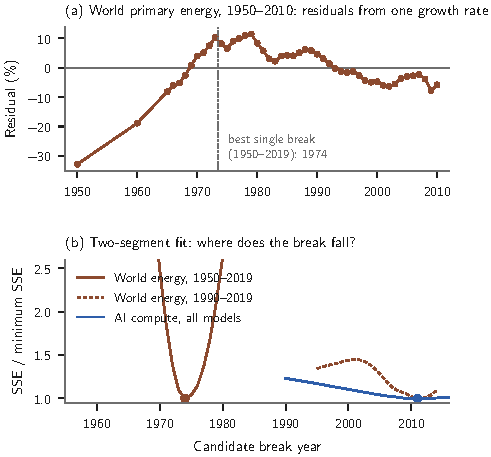
\includegraphics[width=\linewidth]{figs/d2_diagnostics.pdf}
\caption{Fit diagnostics for the growth table. (a) Residuals of world energy around a single 1950--2010 growth rate:
long runs of the same sign (Durbin--Watson 0.15), so the OLS interval is too narrow. (b) Two-segment fits: residual sum
of squares for each candidate break year, relative to the best. World energy breaks in 1974 over 1950--2019, but in
2011 over 1990--2019; AI compute breaks in 2011.}
\label{fig:d2}
\end{figure}

\begin{table}[t]\centering
\caption{Breakpoint tests (two-segment fits). $\Delta$BIC $<0$ favours a break; the more negative, the stronger.}
\label{tab:breaks}
\footnotesize\renewcommand{\arraystretch}{1.1}\setlength{\tabcolsep}{3.6pt}
\begin{tabular}{@{}l l r r l r@{}}
\toprule
Series & Window & $n$ & Break & Before $\to$ after & $\Delta$BIC \\
\midrule
\tabin{tables/breaks.tex}
\bottomrule
\end{tabular}
\end{table}

\paragraph{How far the fits can be trusted (D2 diagnostics)} \Fig{fig:d2} and \Tab{tab:breaks} check the fits behind
\Tab{tab:growth}. Three points stand out. First, the Great Acceleration fit is good ($R^2=0.95$), but its residuals are
strongly autocorrelated (Durbin--Watson 0.15, lag-one correlation 0.93): world energy ran above trend from about 1970 to
the early 1990s and below it after the mid-1990s. The point estimate of 30 years does not change, but an honest interval is 25.6--35.7 years
rather than 27.9--32.0. Second, the compute fit has a tight interval only because it rests on 478 models; individual
models scatter by about 1.7 orders of magnitude around the line ($R^2 = 0.66$), because the list mixes frontier and
smaller models. Third, the breaks are real but depend on the window. AI compute breaks in 2011 with very strong support
($\Delta$BIC $-245$). World energy breaks in 1974, the first oil shock, over 1950--2019 ($-147$), but in 2011 over
1990--2019, with only weak support ($-4$). The 1950 boundary itself cannot be tested, because the series is decadal
before 1965, and the data-centre rows rest on two published points each, so they allow neither an interval nor a break
test.

\begin{reading}
Our reading: the phase boundaries of 1950, 2010 and 2019 are a framing, and the data treat them that way. They support
a break in compute in 2011 and a break in data-centre electricity around 2018, not one clean boundary for everything.
\end{reading}

\begin{figure}[t]\centering
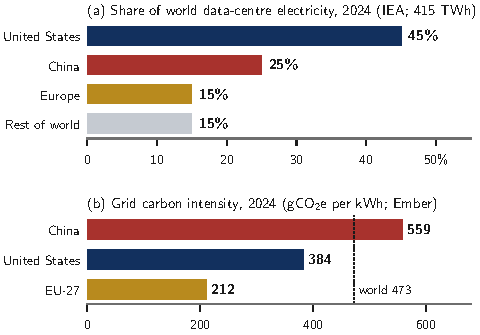
\includegraphics[width=\linewidth]{figs/o1_regional_carbon.pdf}
\caption{Where data-centre electricity is used, and how much \cotwo\ each kWh carries. (a) IEA shares of the
415\,TWh used in 2024. (b) Average grid carbon intensity in 2024 (Ember); the EU-27 stands in for the IEA's
``Europe''. These are grid averages, used as benchmarks, not data-centre emission estimates.}
\label{fig:o1}
\end{figure}

\paragraph{The load is regional; its carbon depends on the grid} Three regions use 85\% of data-centre electricity
(\Fig{fig:o1}). What that electricity emits depends on the grid that supplies it: in 2024 a kWh carried 559\,g of
\cotwo-equivalent in China, 384\,g in the United States and 212\,g in the EU, against a world average of 473\,g
\citep{ember2026}. The same kWh therefore emits about 2.6 times as much in China as in the EU. Electricity is a
regional load, felt by grids and local air; carbon is a global impact, but its size is set by where the load sits.

% 4.2 O2 Materials, water and waste. OWNER: Aryan. Sources: deck slides 21-28 (presentation/analysis/*.py),
% D1 atlas (report/analysis/fig_d1_atlas.py). Numbers: claims.csv rows O2a-O2e, Case1, Case2, Method5; claims_report.csv.
\subsection{O2: Water, materials and waste}\label{sec:o2}

% The atlas is a full-width float: declared here so it lands at the top of the next page.
\begin{figure*}[t]\centering
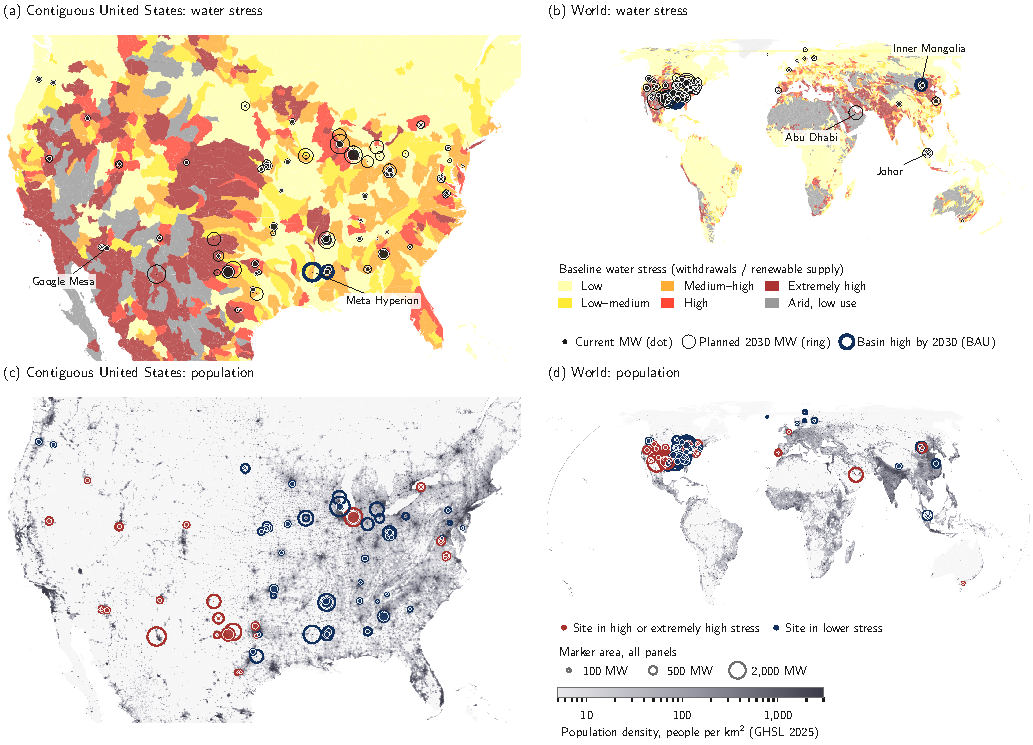
\includegraphics[width=\textwidth]{figs/d1_atlas.pdf}
\caption{Atlas of AI data-centre capacity over water stress and population (deliverable D1). Markers: 96 Epoch AI
sites; filled dot = facility power today, open ring = planned by the end of 2030, area proportional to MW. (a, b) WRI
Aqueduct 4.0 baseline water stress; a thick navy ring marks the four sites whose basin is below ``high'' today but high
or extremely high under the 2030 business-as-usual projection (Meta Hyperion, Amazon Ridgeland and two sites in Inner
Mongolia). (c, d) GHSL 2025 population density; markers are red where the site's basin is in high or extremely high
baseline stress. Grey basins in (a, b) are arid with little water use. Not shown: the Visakhapatnam hub (Section
\ref{sec:cases}), which is not yet in the Epoch data.}
\label{fig:atlas}
\end{figure*}

\paragraph{Where the capacity sits} The 96 sites in the Epoch data add up to 15.1\,GW of facility power today and
50.3\,GW planned by the end of 2030 (\Fig{fig:atlas}). Two things stand out. The rings are much larger than the dots:
most of this capacity is not built yet, so siting decisions are still open. And many of the largest rings sit in red
basins: Stargate in New Mexico, Shackelford and the Texas Panhandle, Stargate UAE in Abu Dhabi, and the Inner Mongolia
cluster. Texas alone plans 7.3\,GW in stressed basins and New Mexico 2.7\,GW. Not every large site is stressed: the
largest planned site, Microsoft's Fairwater campus in Wisconsin (2.7\,GW), sits in a medium--high basin. The population
panels show who lives around these sites: 21 million people within 25\,km of a stressed site (planned sites included),
48 million within 50\,km, out of 106 million within 50\,km of any tracked site.

\begin{figure}[t]\centering
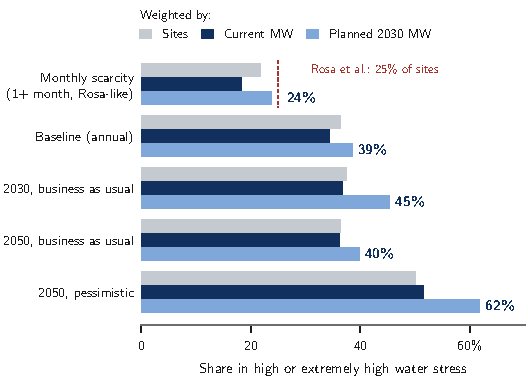
\includegraphics[width=\linewidth]{figs/o2_count_vs_size.pdf}
\caption{Counting sites versus weighting them by size. Share of sites, of current MW and of planned 2030 MW in basins
of high or extremely high water stress, under the baseline and Aqueduct's projections. The red line is Rosa et al.'s
25\%, a share of sites in water-scarce areas.}
\label{fig:count}
\end{figure}

\paragraph{By size, a third of AI capacity is in stressed basins} Counting sites treats a 10\,MW site and a 2\,GW
campus alike, so we weight by power (\Fig{fig:count}). Today 36.5\% of sites and 34.4\% of current MW are in high or
extremely high stress. The planned build-out tilts toward those basins: capacity there grows 3.7-fold to 2030, against
3.1-fold elsewhere, so 38.6\% of the planned MW sits in stressed basins at today's stress levels. Under Aqueduct's 2030
business-as-usual projection the share is 45.4\%. Most of that step comes from two Gulf Coast sites, Meta Hyperion and
Amazon Ridgeland, whose basins sit just under the 40\% line today and cross it in 2030 (+6.4 points); two sites in Inner
Mongolia move from ``arid, low use'' to extremely high (+2.4), and three Utah and Nevada sites drop out ($-1.9$). The
same two Gulf Coast basins fall back by 2050, which is why the 2050 business-as-usual share (39.8\%) is lower than the
2030 one; the 2050 pessimistic case reaches 61.8\%. As a check against Rosa et al.'s monthly method, 21.9\% of our sites
have at least one month in which withdrawals exceed supply, close to their 25\% (2,315 of 9,347 data centres)
\citep{rosa2026}.

\begin{finding}{Finding 2. Weighted by size, 34\% of AI capacity is in stressed basins, 39--45\% of the 2030 plan}
The build-out is heading into dry basins: stressed capacity grows 3.7-fold against 3.1-fold elsewhere. About 21 million
people live within 25\,km of these sites.
\end{finding}

\begin{figure}[t]\centering
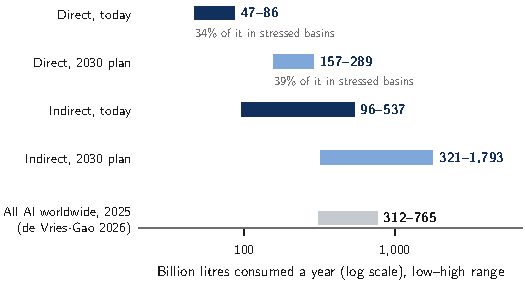
\includegraphics[width=\linewidth]{figs/o2_water_use.pdf}
\caption{Estimated water consumption of the tracked sites, low--high range, today and for the planned 2030 capacity.
Direct: on-site cooling. Indirect: evaporated at the power plants that supply the electricity. Grey: de Vries-Gao's
(2026) estimate for all AI systems worldwide in 2025. Log scale.}
\label{fig:water}
\end{figure}

\paragraph{Most of the water is used at power plants} Today's 15\,GW consume an estimated 143--624 billion litres a
year, and the 2030 plan 478--2,082 billion (\Fig{fig:water}). Between 67 and 86\% of it is \emph{indirect}: water
evaporated at the power plants, not at the data centre. On-site cooling water in stressed basins comes to 16--30
billion litres a year today and 61--111 billion by 2030. Our range for today overlaps de Vries-Gao's independent
estimate of 312--765 billion litres for all AI systems worldwide in 2025 \citep{devriesgao2026}. The width of the range
comes mostly from the grid factor (1.04 against 4.52\,L/kWh). Sites matter more than totals here: the Epoch sites that
report water imply anything from 0.001 to 7\,L per facility kWh (at an assumed 80\% load), against our range of
0.51--0.73\,L for on-site use. Cooling design, not size, decides a site's direct water.

\begin{figure}[t]\centering
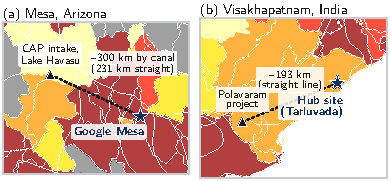
\includegraphics[width=\linewidth]{figs/o2_case_locator.pdf}
\caption{The two case studies and their water sources, over Aqueduct baseline water stress (same colours as
\Fig{fig:atlas}). Star: data centre; triangle: water source. Mesa's Colorado River water reaches the Phoenix area
through the Central Arizona Project canal; Visakhapatnam's promised source is the Polavaram project.}
\label{fig:cases}
\end{figure}

\paragraph{Case 1: Google Mesa, a desert site whose water travels 300\,km}\label{sec:cases} Google's Mesa campus
(183\,MW today, 237\,MW planned) sits in a basin of extremely high stress, where withdrawals exceed renewable supply in
all twelve months of the year. Google's agreement with the city, reported in 2020, guarantees 1 million US gallons a day
and allows up to 4 million, about 15 million litres a day or 5.5 billion litres a year \citep{sattiraju2020,solon2021}.
By our method, on-site use for 237\,MW would be 0.7--1.4 billion litres a year, close to the guaranteed volume (1.4
billion); the ceiling is four to seven times our estimate, so it is a permission, not a measure of use. Actual use is
not disclosed. More than half of Mesa's water (53\%) is Colorado River water delivered through the Central Arizona
Project canal, about 300\,km long (231\,km in a straight line from the intake at Lake Havasu); 40\% comes from the Salt
and Verde rivers and 7\% from groundwater \citep{mesa2026,reclamation_cap}. That river is being cut: in August 2026 the
federal government reduced Lower Basin allocations by 1.25 million acre-feet a year for 2027--2028
\citep{mesa2026,reclamation2026}. Local politics has noticed. When the city approved its next, Facebook-linked data centre in
2021, Vice Mayor Jenn Duff cast the only vote against, calling data centres ``an irresponsible use of our water''
\citep{solon2021}. Her vote concerned that project, not Google's.

\paragraph{Case 2: Visakhapatnam, a gigawatt hub in a city already short of water} Google, with AdaniConneX and
Airtel, plans a 1\,GW AI hub near Visakhapatnam, worth about US\$15 billion \citep{google2025,federal2026}, on three campuses
(Tarluvada, Adavivaram and Rambilli); the foundation stone was laid at Tarluvada on 28 April 2026 \citep{deccan2025,mongabay2026}. The city already receives about 410 of the 480 million litres a day it needs, a
shortfall of 15\% \citep{federal2026}. The environmental clearance does not disclose the site's water use in operation
\citep{mongabay2026}. The state government says water will come by dedicated pipeline from the Polavaram project, about
190\,km away in a straight line, and the companies say the site will be air-cooled; residents have protested under the
slogan ``We cannot drink data'' \citep{federal2026}. Our check places the Tarluvada site in a medium--high stress basin (20--40\%), with no month
in which withdrawals exceed supply. Air cooling removes most of the on-site water, but not the water at the power
plants: for 1\,GW our range is 17--98 million litres a day, equal to 4--24\% of the city's present supply. This compares
scale only. Those plants need not draw on the city's supply, and the grid factors are US-derived. Why this city was chosen,
and whether water stress counted, is the subject of Section~\ref{sec:siting}.

\begin{figure}[t]\centering
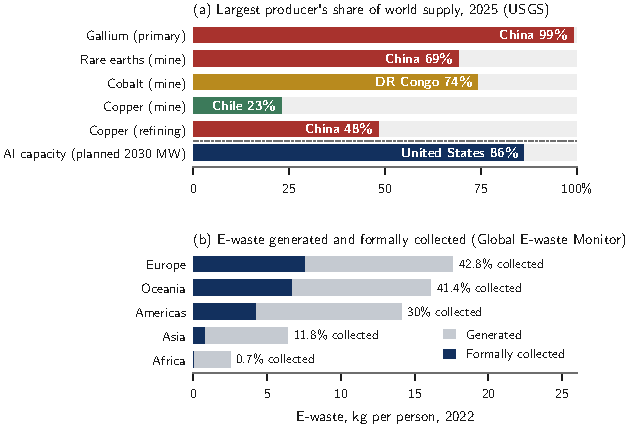
\includegraphics[width=\linewidth]{figs/o2_materials_ewaste.pdf}
\caption{Minerals are mined in a few countries; e-waste collection is very uneven. (a) Share of world supply from
the largest producer, 2025, with the US share of planned AI capacity for comparison. (b) E-waste generated per person
in 2022 and the share formally collected.}
\label{fig:materials}
\end{figure}

\paragraph{Minerals and e-waste} The hardware depends on minerals whose supply is concentrated
(\Fig{fig:materials}). In 2025 China produced 99\% of the world's primary gallium, 69\% of mined rare earths and 48\%
of refined copper; DR Congo mined 74\% of cobalt and Chile 23\% of copper \citep{usgs2026}. The demand sits elsewhere:
86\% of the planned AI capacity in our data is in the United States. Supply can be cut. China's December 2024 ban on
gallium and germanium exports to the United States was suspended under MOFCOM Announcement 72 until 27 November 2026
\citep{usgs2026,mofcom2025}; as of late November 2026 no official notice has extended the suspension (though press reports suggest a possible extension into early 2027), leaving near-term supply uncertain. At the end of the chain, the world
generated 62 million tonnes of e-waste in 2022, of which 22\% was formally collected \citep{balde2024}. Collection
ranges from 42.8\% in Europe to 0.7\% in Africa. The USGS does not break out the share of these minerals that goes
to AI, and the e-waste data cover all electronics, so this part of the analysis shows concentration, not AI's
share.

\paragraph{Against the global boundary} The Earth3 model treats freshwater as one global number: withdrawals below
3,000\,\kmc\ a year are safe, above 4,000\,\kmc\ high-risk \citep{collste2018}. The 2030 plan's 0.5--2.1\,\kmc\ is
0.02--0.07\% of the safe limit. The comparison mixes our consumption with a withdrawal limit, and withdrawals would be
larger, but even several times more would still be well under 1\%.

\begin{finding}{Finding 3. Against a global boundary AI's water barely registers; in a basin it does}
Under 0.1\% of Earth3's freshwater limit, yet 12 of 12 months over supply in Mesa's basin, and a planned gigawatt hub
in a city already 15\% short. A single global number averages away exactly where the pressure is: AI's water has to be
judged basin by basin.
\end{finding}

% 4.3 Siting logic: why Visakhapatnam? Added after the first draft. Extends Case 2 of O2 (sec:cases).
% Sources: public statements, official documents and press only (refs.bib: afp2026, google2026env, mongabay2026,
% scroll2026, tnm2026, newsminute2025, csm2026, niti2026, theprint2026, ceew2026, deccan2025, bs2026, googlewater2026).
% Our numbers: report/analysis/fig_siting.py -> figs/o2_siting.pdf, data/o2_siting_airwater.csv; logged in claims_report.csv (4.3).
\subsection{Siting logic: why Visakhapatnam?}\label{sec:siting}

Case~2 (Section~\ref{sec:cases}) leaves a question that the water data cannot answer. If Visakhapatnam is already
short of water, why was it chosen? We ask three things. What reasons did the project's backers give? Did water stress, the
distance to the water source or the people living nearby enter the decision? And was there a framework that required them
to? We rely on public statements, official documents and press reports only, so we can say what was stated and what is on
the record, not what was weighed in private.

\paragraph{The stated reasons are connectivity, power, talent and policy} Google told AFP that it looks for proximity to
customers and users, access to talent, potential for new clean energy and partnerships with local communities, and that
Visakhapatnam is ``one of the few places where all of these come together''; the coast also lets undersea cables reach
Australia and South Africa, making Andhra Pradesh ``India's third major subsea hub'' \citep{afp2026}. The
company's own announcement presents the cable gateway as route diversity beside the existing landings in Mumbai and Chennai
\citep{google2025}. The state added fiscal reasons: a 25\% discount on land, a 25\% discount on the price of industrial water
supply, exemption from electricity duty and a lower power tariff \citep{newsminute2025}, which the Wall Street Journal values at about
US\$2.3 billion over 20 years \citep{csm2026}. Scale matters too. India's installed data-centre capacity was about 1.5\,GW in
mid-2025 \citep{ceew2026}, so a 1\,GW hub is equal to two-thirds of it. Nor is the hub one site: it is planned on three
campuses, at Tarluvada, Adavivaram and Rambilli \citep{deccan2025}. Our case study uses Tarluvada, where the foundation stone was laid.

\paragraph{Water came in as a design input, not as a siting test} Google says independent assessments of grid stability,
power supply, water risk, ecology and noise are made 12 to 24 months before a project starts, and that the water assessment for
Visakhapatnam ``pointed to pressure on the local watershed'', which ``shaped our choice of cooling configuration from the
outset'': advanced air cooling instead of water \citep{afp2026}. That fits Google's published water-risk framework, which
rates a site's watershed for scarcity and depletion and turns to air cooling or recycled water where risk is high
\citep{google2026env}. Three things follow. First, the selection criteria Google listed to AFP do not name water; the water finding is
reported as acting on the cooling design, not on the location. Second, none of it can be checked. Google reports water use
only for fully operational sites \citep{csm2026}, and the environmental clearance discloses neither the water used in operation nor its source
\citep{mongabay2026}. Petitioners call the assessments ``inadequate'' \citep{bs2026}; we cannot confirm or refute that.
Third, the state treats water as a price: a discount, and a promise of supply by dedicated pipeline from the Polavaram
project, about 190\,km away in a straight line. An assessment of the \emph{local} watershed says nothing about water
drawn from elsewhere, whether for non-cooling needs or at the power plants (Section~\ref{sec:o2}).

\paragraph{Water stress was seen, but as a risk to manage} The record is mixed. By the Aqueduct measure Visakhapatnam is not an
extreme site: its basin is medium--high (20--40\%), with no month in which withdrawals exceed supply, and basins hosting
37.5\% of the planned capacity in our sample are less stressed while 38.6\% are more stressed (\Fig{fig:siting}a). But the
city already receives 410 of the 480 million litres a day it needs, and the district had the lowest groundwater availability in
the state (2.12\,TMC) on 1 April 2026 \citep{scroll2026}. Across India, a CEEW study found that most industry stakeholders rate water risk as low to medium, even though data
centres cluster in Mumbai, Hyderabad, Chennai and Bengaluru, where urban water demand is already high \citep{ceew2026}.
Water stress is therefore \emph{seen}, but as one risk among several rather than a reason to choose another place.

\begin{figure}[t]\centering
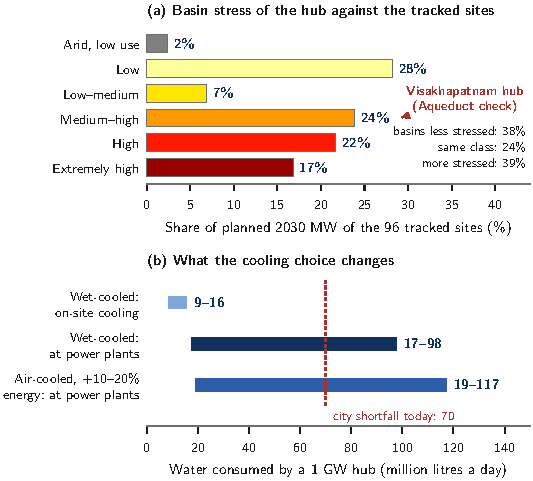
\includegraphics[width=\linewidth]{figs/o2_siting.pdf}
\caption{(a) Planned 2030 MW of the 96 tracked sites by Aqueduct baseline water-stress class, with the class of the Visakhapatnam
hub's basin (our check at Tarluvada; the hub is not in the Epoch data). (b) Water consumed by a 1\,GW hub with the Section~\ref{sec:methods}
model (low--high range): on-site cooling if wet-cooled; the water evaporated at the power plants; and the same if air cooling
needs 10--20\% more energy. Dashed line: the city's shortfall today (480 minus 410 million litres a day). US-derived grid
factors; the load factor is our assumption.}
\label{fig:siting}
\end{figure}

\paragraph{Distance and population are not criteria anywhere} We found no framework, statement or document in which the distance from a
site to its water source or the number of people nearby is a stated test. Distance enters only through the pipeline. Population
enters through public process, and there the record is thin: Mongabay India quotes a campaigner saying that data centres are being appraised as
building or township projects, which need neither a public hearing nor a draft environmental impact report. The State Environment
Impact Assessment Authority cleared the Tarluvada project on 18 April 2026, nine days after the application \citep{mongabay2026,tnm2026}. The News Minute
adds that the clearance itself records that nearly 90\% of the Tarluvada site lies in a reserve forest \citep{tnm2026}.

\begin{table*}[t]\centering
\caption{Instruments that could have governed the siting of the Visakhapatnam hub, and whether they tested water.}
\label{tab:frameworks}
\footnotesize\renewcommand{\arraystretch}{1.1}
\begin{tabular}{@{}P{3.6cm}P{4.4cm}P{8.3cm}@{}}
\toprule
Instrument & Status when the site was chosen & What it asks about water and siting \\
\midrule
Draft National Data Centre Policy (MeitY, 2020) & Never notified & No binding environmental requirement
\citep{mongabay2026} \\
State data-centre policies (15 states) & In force & Most set no PUE or WUE standard \citep{mongabay2026} \\
Environmental clearance (EIA Notification 2006) & Applied (18 April 2026) & Appraised as a building or township project (as reported): no public hearing;
operating water use and source not disclosed \citep{mongabay2026,tnm2026} \\
Google's water-risk framework & Company-internal; results not published & Rates the local watershed; high risk points to
air cooling or recycled water \citep{google2026env,afp2026} \\
NITI Aayog and Deloitte \emph{Data Centre Evaluation Framework} & Released 14 October 2026, after approval and groundbreaking; advisory
& Five pillars, including water and siting. A 20--30-year seasonal water balance for each catchment, including farming; ``red zones''
for water stress; MeitY audit; states apply it \citep{niti2026,theprint2026} \\
\bottomrule
\end{tabular}
\end{table*}

\paragraph{Frameworks exist, but none was in force in time} Several exist (\Tab{tab:frameworks}), but none was binding when the site was chosen, and the only
one that tests catchment water, the NITI Aayog evaluation framework, arrived in October 2026, six months after the clearance
and the groundbreaking. Visakhapatnam was not judged against it. Its tests are the ones this section found missing: a water
balance that counts competing users, restricted zones where stress is high, and checks on who benefits.

\paragraph{What the cooling choice changes} Air cooling does remove the water that would be evaporated on site. By our
model that is 9--16 million litres a day for 1\,GW, 2--4\% of the city's present supply (\Fig{fig:siting}b). But air cooling needs more
electricity, about 10\% on average and roughly twice that on a hot day by Google's own figure \citep{googlewater2026}, and
most of the hub's water is used at the power plants anyway. With 10--20\% more energy the water at the power plants rises by 2--20
million litres a day, so the net effect on all water consumed lies between a saving of 7 and an increase of 4 million litres a day. In
Google's words, ``it becomes a tradeoff between reducing stress on the grid versus reducing stress on the watershed''
\citep{googlewater2026}. Air cooling therefore mostly \emph{moves} the water from the city to the power stations, and the
carbon to the grid. It protects the town's taps, which matters locally, but it is not a net water saving.

\begin{reading}
Our reading: on the public record, connectivity, power, land and incentives chose the site, and water was handled afterwards,
through the choice of cooling, a pledge to replenish, and a pipeline. That is a defensible design response, and the site is not
the most stressed in our sample. But it leaves the questions a water-first screen would ask (distance to source, competing
users, the people nearby) unanswered in public, and no framework in force required them. A comparison with Mumbai, Chennai,
Hyderabad and Bengaluru would show whether Visakhapatnam was the better water choice among Indian options.
\end{reading}

\begin{finding}{Finding 4. Water shaped how Visakhapatnam will be cooled, not whether it was chosen}
On the public record the site was chosen for cables, power, land and incentives; water risk acted on the cooling design.
Distance to source and nearby population are tests in no instrument in force at the time, and the first framework that
asks for a catchment water balance (NITI Aayog, October 2026) came after the clearance. Air cooling shifts, rather than removes,
the hub's water: net change between $-7$ and $+4$ million litres a day.
\end{finding}

% 4.3 O3 Economy, politics and society. OWNER: Prerna. First draft by Aryan from the deck (slides 30-31) and the D3
% country table (report/analysis/d3_country_table.py). Numbers: claims.csv rows O3, S5/O3; claims_report.csv.
\subsection{O3: Economy, politics and society}\label{sec:o3}

\begin{table*}[t]\centering
\caption{Country table (deliverable D3): the 12 countries with a tracked AI site. MW: facility power today and planned
by the end of 2030. Population: GHSL 2025 (world: 8.19 billion). $LQ$: share of capacity $\div$ share of world
population (``--'': no capacity yet). Stressed: share of the country's planned MW in basins of high or extremely high
baseline stress. People: within 50\,km of any of the country's sites, counted once; Malaysia's Johor sites include
residents of Singapore. Water: our low--high consumption range for the planned capacity, direct plus indirect.
Country-level Gini of capacity per person: 0.936 today, 0.940 for the 2030 plan.}
\label{tab:d3}
\footnotesize\renewcommand{\arraystretch}{1.08}\setlength{\tabcolsep}{3.7pt}
\begin{tabular}{@{}l r r r r r r r r r r r@{}}
\toprule
 & & \multicolumn{2}{c}{MW} & Share of & Population & \multicolumn{2}{c}{$LQ$} & W per person & Stressed & People
 & Water 2030 \\
\cmidrule(lr){3-4}\cmidrule(lr){7-8}
Country & Sites & today & 2030 & 2030 MW (\%) & (M) & today & 2030 & (2030) & (\% of MW) & $\le$50\,km (M) & (bn L/yr) \\
\midrule
\tabin{tables/d3_country.tex}
\bottomrule
\end{tabular}
\end{table*}

\paragraph{Capacity is far more concentrated than people} The United States holds 83.4\% of the 15,078\,MW tracked
today and 86.2\% of the 2030 plan, with 4.2\% of the world's population (\Tab{tab:d3}). Its location quotient is
therefore about 20: twenty times its population share. Malaysia, with several large sites in Johor next to Singapore,
has almost the same quotient today (19.5), falling to 9.2 by 2030 as US capacity grows faster. The highest 2030 quotient
belongs to the United Arab Emirates (24.0), where one planned 1.4\,GW campus serves 9.5 million residents. The Nordic
countries and Iceland sit between 4 and 8, reflecting a few sites in small populations. At the other end, China hosts
5.9\% of today's tracked capacity with 17.4\% of the world's people ($LQ$ 0.34) and Indonesia 0.5\% with 3.4\% (0.14).
The 2030 plan works out at 127\,W per person in the United States against a world average of 6.1\,W, and 73\% of
the world's people live in countries with no tracked AI site at all.

\begin{figure}[t]\centering
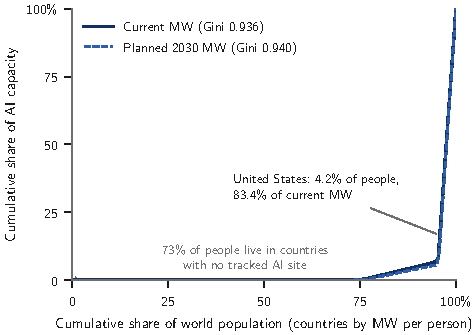
\includegraphics[width=\linewidth]{figs/o3_lorenz.pdf}
\caption{Lorenz curve of tracked AI capacity against population, by country (deliverable D3). Countries are sorted
by MW per person; the diagonal would be perfect equality. Countries without a tracked site are pooled at zero, which
leaves the Gini unchanged.}
\label{fig:lorenz}
\end{figure}

\paragraph{The country-level Gini} The Lorenz curve (\Fig{fig:lorenz}) hugs the bottom axis until the last few
percent of the world's population. The Gini coefficient of capacity per person is 0.936 for current capacity and 0.940
for the 2030 plan. The presented deck reported 0.927 from seven country groups (with UN population data,
\citealp{undesa2024}); pooling
countries inside groups hides inequality within them, so the group value is a lower bound, and the country-level value
is indeed higher. Among the host countries alone the Gini is 0.76 (0.78 for 2030): even among countries that host AI
capacity, it is very unevenly spread. Both values describe the Epoch sample, which is AI-only and US-heavy (Section
\ref{sec:limits}); they measure where large AI campuses are being built, not all digital infrastructure.

\paragraph{Water stress and exposure by country} The country view also shows where the water pressure of
Section~\ref{sec:o2} lands. In the United States 39\% of the planned capacity is in stressed basins, and 68 million
people live within 50\,km of a site. China's share is 24\%; Malaysia's sites are all in lower-stress basins. Four
countries (the UAE, Portugal, the United Kingdom and Australia) have a single site each, all in stressed basins, so
their 100\% is one site, not a pattern.

\paragraph{Local opposition is rising} In the United States, organised opposition is now common. Data Center Watch
counts at least 75 projects worth about US\$130 billion blocked or delayed in the first quarter of 2026, with the
number of active opposition groups more than doubled since the end of 2025 and present in 49 states \citep{dcw2026}.
The second quarter eased but stayed high: at least 45 projects worth about US\$68 billion, and 843 opposition groups, up from 833
at the end of March \citep{dcw2026q2}.
We code disputes with five grievance tags adapted from the EJAtlas \citep{temper2015}: \emph{water} (cooling
withdrawals, basin stress, competition with households and farms), \emph{power} (grid connection, new generation,
electricity bills, fossil lock-in), \emph{noise} (fans, chillers, backup generators), \emph{land} (campus footprint,
rezoning, habitat) and \emph{jobs} (construction against permanent jobs). This is a coding framework, not a measured
total; both of our case studies are water disputes. Supply-chain concentration, the third part of O3, is shown in
\Fig{fig:materials}: the minerals come from a few countries, and one export ban can reach the whole build-out.

\begin{finding}{Finding 5. Capacity per person is twenty times the world share in the US and Malaysia}
Country-level Gini 0.94: 73\% of the world's people live in countries with no tracked AI site. The concentration that
makes AI's footprint small globally is what makes it large locally.
\end{finding}

% 4.4 O4 Synthesis (all). Source: deck slide 33 (evidence-coded matrix), with Q/D/N codes kept as presented.
\subsection{O4: Synthesis by boundary and scale}\label{sec:o4}

\begin{table*}[t]\centering
\caption{Each pressure has its own scale. Planetary boundaries against the scale of impact of AI data centres.
\textbf{Q}: quantified in this project; D: documented pathway, not quantified; N: not assessed. Status is the 2025
global assessment of all human activity \citep{sakschewski2025}, not a finding that data centres caused it.}
\label{tab:matrix}
\footnotesize\renewcommand{\arraystretch}{1.12}
\begin{tabular}{@{}P{2.35cm}P{1.7cm}P{3.75cm}P{3.75cm}P{3.75cm}@{}}
\toprule
Boundary & Status (2025) & Local & Regional & Global \\
\midrule
Climate change & Transgressed & D\enspace Backup generators; construction & \textbf{Q}\enspace Grid intensity 212--559\,g
\cotwo/kWh (\Fig{fig:o1}) & D\enspace Operational and embodied greenhouse gases \\
Freshwater change & Transgressed & \textbf{Q}\enspace 34\% of capacity in stressed basins; Mesa up to 15\,M\,L/day
& \textbf{Q}\enspace 67--86\% of water used at power plants & \textbf{Q}\enspace $<$0.1\% of Earth3's limit: the
total hides the hotspots \\
Land-system change & Transgressed & D\enspace Campus and substation footprint & D\enspace Transmission corridors;
mining land & D\enspace Land conversion in the supply chain \\
Biosphere integrity & Transgressed & D\enspace Habitat effects of sites & D\enspace Mining, river and wetland pressure &
D\enspace Cumulative ecosystem pressure \\
Biogeochemical flows & Transgressed & N & D\enspace Generation, mining and runoff & N \\
Novel entities & Transgressed & D\enspace Refrigerants, chemicals, exhaust & \textbf{Q}\enspace E-waste collected:
42.8\% in Europe, 0.7\% in Africa & D\enspace Hazardous material flows \\
Ocean acidification & Transgressed & N & N & D\enspace Through \cotwo\ only \\
Aerosol loading & Safe & D\enspace Diesel and construction particulates & D\enspace Combustion pollution & N \\
Stratospheric ozone & Safe & N & N & N \\
\bottomrule
\end{tabular}
\end{table*}

\Tab{tab:matrix} brings the four objectives together. The strongest evidence is for freshwater, which we quantified
at all three scales: locally (a third of capacity in stressed basins, and Mesa's contract), regionally (most of the
water is evaporated at power plants on the regional grid) and globally (a negligible share of the planetary limit,
which is itself the finding). Climate change acts through the grid: the load is regional and the carbon intensity is set
regionally, but the emissions add to a global stock. Minerals and e-waste move through global supply chains, so their
impacts are displaced: mined in one region, used in a second and discarded in a third. Most other cells are documented
pathways that we did not measure; we mark them as such rather than fill them. The siting audit adds who decides:
at Visakhapatnam no instrument in force required a water test before the site was chosen (Section~\ref{sec:siting}), so the
local water pressure shown in the matrix was not tested at the site before approval.

\begin{reading}
Our reading: the matrix also shows why a safe-and-just view \citep{rockstrom2023} matters for this topic. A boundary
defined only by the global total says AI's water is safe. A boundary that asks who is harmed points to the 21 million
people near stressed sites, a desert city on a shrinking river, and a port city already short of drinking water.
\end{reading}

\begin{finding}{Finding 6. Small globally, concentrated locally}
AI's footprint is a small share of the world's electricity and water, but it piles up in a few countries, grids,
basins and towns. Each pressure has its own scale, and each scale needs its own response.
\end{finding}

% 5 Deliverables (all). What was promised in the plan (section 5) against what was delivered. Source: deck slide 35,
% updated for what the report adds. Keep the D2 status "Partly complete" unless the data-centre rows get real fits.
\section{Deliverables}\label{sec:deliverables}

\Tab{tab:deliv} sets each promised deliverable against what this report contains. The report completes the pieces
the presentation deferred (the atlas, the country table with location quotients and a country-level Gini, and fit
diagnostics for the growth table), except where the data do not allow it.

\begin{table}[t]\centering
\caption{Deliverables: plan against delivery.}
\label{tab:deliv}
\footnotesize\renewcommand{\arraystretch}{1.12}\setlength{\tabcolsep}{4pt}
\begin{tabular}{@{}l P{2.05cm} P{3.55cm} P{1.45cm}@{}}
\toprule
 & Promised & Delivered & Status \\
\midrule
D1 & Atlas of capacity over water stress and population, with 2030 & \Fig{fig:atlas}: capacity, stress and population
on the same maps, US and world; 2030 capacity and 2030 stress transitions marked & \textbf{Complete} \\
D2 & Growth table (\%/yr, doubling time, 95\% intervals) for the three phases & \Tab{tab:growth}, with OLS and HAC
intervals, $R^2$ and break tests (\Tab{tab:breaks}, \Fig{fig:d2}). Data-centre rows: two published points, no
interval or break test & \textbf{Partly complete} \\
D3 & Regional table: LQ, Gini, size-weighted stress, exposed population, water use & \Tab{tab:d3}: 12 countries,
LQ today and 2030, country Gini, stress, people within 50\,km, water. Population from GHSL, not WPP; no Gini per
internet user & \textbf{Complete} (country level) \\
D4 & Case profiles; boundary $\times$ scale matrix with responses; final report & Mesa and Visakhapatnam
(Section~\ref{sec:cases}) and a siting audit of the second (Section~\ref{sec:siting}); \Tab{tab:matrix}; responses in Section~\ref{sec:responses}; this report &
\textbf{Complete} (draft) \\
\bottomrule
\end{tabular}
\end{table}

\paragraph{Corrections carried over from verification} Before the presentation every number was checked against its
source and logged. Four corrections from that check stand in this report. The EU grid carbon intensity is 212\,g/kWh
(Ember 2024), not the 179\,g in an earlier draft. A claim of ``833 opposition groups'' could not be found on the Data
Center Watch Q1 page and was dropped from the deck; press coverage of the Q2 report later gave 833 as the end-of-March count,
so the number was right but the source was wrong, and we now cite the Q2 report. Vice Mayor Duff's 2021 vote concerned a Facebook-linked data centre, not Google's.
Epoch AI's capacity figures are facility power, not IT power, and every figure is labelled accordingly. Two more
corrections are new in the report. One of the two Inner Mongolia sites that enter extreme stress by 2030 is in Horinger
(Hohhot), not Ulanqab as the deck's notes put it. And the Visakhapatnam hub is planned on three campuses (Tarluvada,
Adavivaram and Rambilli), not at Tarluvada alone as the deck's slides implied; our basin check is for Tarluvada.

% 6 Summary and conclusions (all). Verdicts as presented (deck slide 37): keep them unless new evidence changes them.
\section{Summary and conclusions}\label{sec:conclusions}

\subsection{What we expected, and what we found}
The plan stated three expected results. \Tab{tab:verdicts} sets each against the evidence. The first is only
\emph{partly confirmed}: concentration is now confirmed at country level (Gini 0.94), but the claim that capacity sits
far from its water source rests on two case studies, not a systematic measurement. The second, the efficiency
explanation, is \emph{partly supported}: the timing fits the end of building-efficiency gains, but chip efficiency was
not tested. The third is \emph{supported as a framework}: impacts do sort by scale, but several cells of the matrix are
documented rather than measured.

\begin{table}[t]\centering
\caption{Expected results (from the plan) against what we found.}
\label{tab:verdicts}
\footnotesize\renewcommand{\arraystretch}{1.15}
\begin{tabular}{@{}P{2.0cm}P{3.75cm}P{1.6cm}@{}}
\toprule
Expected & Found & Verdict \\
\midrule
Capacity is far more concentrated than population; part of it sits in water-stressed basins, often far from its
water source & 83\% of tracked AI power is in the US; country Gini 0.94; LQ about 20 in the US and Malaysia. 34\% of
capacity in high-stress basins today, 39--45\% of the 2030 plan. Distance to source shown for two cases only (231 and
193\,km in a straight line) & \textbf{Partly confirmed} \\
Cloud-era growth was absorbed by one-off efficiency gains, now used up, so AI-era growth outpaces efficiency &
Compute broke upward in 2011, yet data-centre electricity rose only 6\% in 2010--18. PUE flat since 2014; the post-2018
jump (7 to 18\% a year) matches AI-server demand ($<$2 to $>$40\,TWh). Chip efficiency not tested & \textbf{Partly
supported} \\
Electricity and water impacts are local or regional; carbon is global; minerals and e-waste are displaced & Water:
$<$0.1\% of the global limit, but 12 of 12 months over supply in Mesa's basin. Grid carbon varies 2.6-fold. Minerals
come from a few producers; e-waste collection is very uneven (0.7--42.8\%) & \textbf{Supported as a framework} \\
\bottomrule
\end{tabular}
\end{table}

\subsection{Limitations}\label{sec:limits}
The findings are only as good as the data behind them. In rough order of how much they matter:
\begin{enumerate}[leftmargin=1.3em,itemsep=1.5pt]
\item \textbf{The sample is AI-only and US-heavy.} Epoch AI tracks 96 large AI sites, 77 of them in the United States.
It is not a census of data centres: the IEA's 415\,TWh covers all of them. Shares, the Gini and the location quotients
describe where large AI campuses are being built, and countries such as India appear only through a case study.
\item \textbf{Water stress counts power-plant withdrawals.} Aqueduct's annual stress is total withdrawals over renewable
supply, and withdrawals include thermoelectric cooling water, most of which is returned. Basins with large power plants,
such as parts of Indiana and western New York, probably score ``high'' partly for that reason.
\item \textbf{Consumption against a withdrawal limit.} Our water figures are consumption; Earth3's freshwater boundary is
set on withdrawals. The comparison is conservative (withdrawals would be larger), but the two are not the same
quantity.
\item \textbf{US-derived grid water factors.} The indirect range uses 1.04--4.52\,L/kWh, from IEA- and LBNL-based values
that reflect the US grid. Applying them to India (Visakhapatnam) or Malaysia is an approximation; local generation mixes
could give lower or higher values.
\item \textbf{The load factor is assumed.} We assume sites draw 70--90\% of facility power on average. No site reports
this, and partly built campuses may run lower; water scales linearly with it.
\item \textbf{The seven-group Gini was a lower bound.} The deck's 0.927 pooled countries; our country-level 0.94 is the
exact value for the sample. It still cannot see inequality within countries.
\item \textbf{Breakpoints depend on the window.} World energy breaks in 1974 over 1950--2019 but in 2011 over
1990--2019, and 1950 cannot be tested because earlier data are decadal.
\item \textbf{Data-centre growth rests on published points.} Each data-centre row of \Tab{tab:growth} rests on two
published values, not a series we fitted, so it has no interval; the US rates are those stated by LBNL. Masanet et al.'s
+6\% is taken from the LBNL summary of the paper.
\item \textbf{The siting reading rests on public sources.} Section~\ref{sec:siting} uses statements, official documents and press reports,
some from campaigners and some from the company; Google's water assessment for Visakhapatnam is unpublished. Our air-cooling arithmetic uses
US-derived grid factors and a 10--20\% energy penalty taken from a company statement. We did not compare Visakhapatnam with other Indian hubs.
\item \textbf{Facility versus IT power.} Epoch's MW are facility power; we convert to IT energy with the PUE range. Sites
that report water do not state the basis, so the 0.001--7\,L/kWh spread is indicative only.
\end{enumerate}

\subsection{Responses matched to the scale of impact}\label{sec:responses}
Because each pressure has its own scale, no single policy covers them.
\textbf{Locally}, siting rules can keep large campuses out of basins in extreme stress or require non-potable water
(reclaimed or treated wastewater), and permits can cover noise and diesel backup generators. Approval could also require a
published catchment water balance, the water source and its distance, and a public hearing, tests that the Visakhapatnam record
lacks and that the NITI Aayog framework now proposes (Section~\ref{sec:siting}).
\textbf{Regionally}, grid planning and fair tariffs can stop households paying for data-centre load, and water can be
allocated by river basin, so that a city's supply and a power plant's cooling are judged together.
\textbf{Globally}, mandatory disclosure of energy, water and location-based carbon (from the actual local grid, not
offset by certificates bought elsewhere), site by site, would close most of the data gaps listed above, and
supply-chain standards can address mineral concentration and the e-waste collection gap.

\subsection{Conclusion}
The cloud era showed that computing can grow without much more electricity, as long as buildings keep getting more
efficient. That margin ran out around 2014, and the AI build-out arrived after it: compute took off in 2011, electricity
followed after 2018. Its footprint is still small against global totals (1.5\% of electricity, under 0.1\% of the
freshwater boundary), and that is exactly why global totals are the wrong yardstick. Weighted by size, a third of AI
capacity already sits in water-stressed basins and nearly half of the 2030 plan could; most of its water is evaporated
at power plants; and the capacity itself is concentrated in a handful of countries, with a Gini of 0.94. AI does not
have one footprint. It has a local, a regional and a global one, and each needs its own response.


\bibliographystyle{apalike}
\bibliography{refs}
% Printed after the bibliography (small type, as in the reference format).
\par\medskip\noindent{\footnotesize\textbf{Sources of numbers and figures.} Every number in this report is either cited
above or computed by our own scripts; each is logged with its source and method in \texttt{claims.csv} (presented deck)
and \texttt{claims\_report.csv} (new in this report). All figures and tables are our own, drawn from the scripts in
\texttt{report/analysis/}. Base maps: WRI Aqueduct 4.0 and GHSL GHS-POP; site locations from Epoch AI geocoded with
OpenStreetMap.\par}

% Author contributions
\section*{Author contributions}
{\footnotesize
\begin{description}[leftmargin=0pt,labelsep=0.4em,itemsep=3pt]
\item[Aditya Kumar:] Energy and carbon (Objective~O1); creation of presentation; research, finding sources and reports.
\item[Aryan Solanki:] Water, materials and waste (Objective~O2); creation of report; research.
\item[Prerna Sawane:] Economy, politics and society (Objective~O3); proof reading.
\end{description}
\par\medskip\noindent
All authors contributed to the synthesis (Objective~O4) and reviewed the final report.\par}


\end{document}
